\documentclass[UTF8,a4paper,10pt,nocolorlinks]{ctexart}
\usepackage[left=2.50cm, right=2.50cm, top=2.50cm, bottom=2.50cm]{geometry} %页边距
\CTEXsetup[format={\Large\bfseries}]{section} %设置章标题居左   


\usepackage{setspace}
\usepackage{xcolor}
\usepackage{mdframed}
\usepackage{titletoc}
\usepackage{etoolbox}
%%%%%%%%%%%%%%%%%%%%%%%
% -- text font --
% compile using Xelatex
%%%%%%%%%%%%%%%%%%%%%%%
% -- 中文字体 --
%\setmainfont{Microsoft YaHei}  % 微软雅黑
%\setmainfont{YouYuan}  % 幼圆    
%\setmainfont{NSimSun}  % 新宋体
%\setmainfont{KaiTi}    % 楷体
%\setmainfont{SimSun}   % 宋体
%\setmainfont{SimHei}   % 黑体
% -- 英文字体 --
%\usepackage{times}
%\usepackage{mathpazo}
%\usepackage{fourier}
%\usepackage{charter}
\usepackage{helvet}
\usepackage{caption}
\usepackage{multicol} %用于实现在同一页中实现不同的分栏
\usepackage{changepage}
\usepackage{graphics}
\usepackage{amsmath, amsfonts, amssymb} % math equations, symbols
\usepackage[english]{babel}
\usepackage{color}      % color content
\usepackage{graphicx}   % import figures
\usepackage{url}        % hyperlinks
\usepackage{bm}         % bold type for equations
\usepackage{multirow}
\usepackage{booktabs}
\usepackage{epstopdf}
\usepackage{epsfig}
\usepackage{algorithm}
\usepackage{algorithmic}
\newcommand{\sihao}{\fontsize{14pt}{\baselineskip}}
\renewcommand{\algorithmicrequire}{ \textbf{Input:}}     % use Input in the format of Algorithm  
\renewcommand{\algorithmicensure}{ \textbf{Initialize:}} % use Initialize in the format of Algorithm  
\renewcommand{\algorithmicreturn}{ \textbf{Output:}}     % use Output in the format of Algorithm  
\renewcommand{\figurename}{图}
% 引用参考文献标号显示在右上角
\newcommand{\upcite}[1]{\textsuperscript{\textsuperscript{\cite{#1}}}}
% \hypersetup{colorlinks=false} 
% \usepackage{fancyhdr} %设置页眉、页脚
% %\pagestyle{fancy}
% \lhead{}
% \chead{}
% %\rhead{\includegraphics[width=1.2cm]{fig/ZJU_BLUE.eps}}
% \lfoot{}
% \cfoot{}
% \rfoot{} 
\usepackage{color}
\usepackage{subfigure}
\usepackage{changepage}
\usepackage{fancyhdr} %设置页眉、页脚
\pagestyle{fancy}  %%%单线页眉
\fancyhead{}
\fancyhead[LO]{chapter 5}
\fancyhead[RO]{fengxuewei}
% \fancyfoot[RO]{\thepage}
\fancypagestyle{plain}{%
  \pagestyle{fancy}
}
\usepackage{shorttoc}
\usepackage{xcolor}
\usepackage{mdframed}
\usepackage{titletoc}
\renewcommand{\today}{\CJKnumber\year 年 \CJKnumber\month 月 \CJKnumber\day 日}

\DeclareRobustCommand{\chuhao}{\fontsize{42pt}{\baselineskip}\selectfont}  % 初号
\DeclareRobustCommand{\xiaochu}{\fontsize{36pt}{\baselineskip}\selectfont} % 小初
\DeclareRobustCommand{\yihao}{\fontsize{26pt}{\baselineskip}\selectfont}   % 一号
\DeclareRobustCommand{\xiaoyi}{\fontsize{24pt}{\baselineskip}\selectfont}  % 小一
\DeclareRobustCommand{\erhao}{\fontsize{22pt}{\baselineskip}\selectfont}   % 二号
\DeclareRobustCommand{\xiaoer}{\fontsize{18pt}{\baselineskip}\selectfont}  % 小二
\DeclareRobustCommand{\sanhao}{\fontsize{16pt}{\baselineskip}\selectfont}  % 三号 
\DeclareRobustCommand{\xiaosan}{\fontsize{15pt}{\baselineskip}\selectfont} % 小三
\DeclareRobustCommand{\sihao}{\fontsize{14pt}{\baselineskip}\selectfont}   % 四号
\DeclareRobustCommand{\xiaosi}{\fontsize{12pt}{\baselineskip}\selectfont}  % 小四
\DeclareRobustCommand{\wuhao}{\fontsize{10.5pt}{\baselineskip}\selectfont} % 五号
\DeclareRobustCommand{\xiaowu}{\fontsize{9pt}{\baselineskip}\selectfont}   % 小五
\DeclareRobustCommand{\liuhao}{\fontsize{7.5pt}{\baselineskip}\selectfont} % 六号
\DeclareRobustCommand{\xiaoliu}{\fontsize{6.5pt}{\baselineskip}\selectfont}% 小六
\DeclareRobustCommand{\qihao}{\fontsize{5.5pt}{\baselineskip}\selectfont}  % 七号

\providecommand{\keywords}[1]{\textbf{\textit{keywords---}} #1}
%%%%%%%%%%%%%%%%%%%%%%%
%  设置水印
%%%%%%%%%%%%%%%%%%%%%%%
%\usepackage{draftwatermark}         % 所有页加水印
%\usepackage[firstpage]{draftwatermark} % 只有第一页加水印
% \SetWatermarkText{Water-Mark}           % 设置水印内容
% \SetWatermarkText{\includegraphics{fig/ZJDX-WaterMark.eps}}         % 设置水印logo
% \SetWatermarkLightness{0.9}             % 设置水印透明度 0-1
% \SetWatermarkScale{1}                   % 设置水印大小 0-1    
 
\usepackage{hyperref} %bookmarks

\captionsetup[figure]{labelfont={bf},labelformat={default},labelsep=period,name={图}}
\hypersetup{colorlinks, bookmarks, unicode} %unicode

\title{
    \textbf{chapter 5. Linear Design Models}\\
    \textbf{线性设计模型}
}
\author{ fengxuewei }
\date{\today}
\begin{document}
    \maketitle
    
    % \begin{itemize}
    %     \item[(1)] 介绍连续闭环(SLC)方法
    %     \item[(2)] 执行器饱和度 saturation 及其对性能的限制
    %     \item[(3)] 横向自动飞行器的设计
    %     \item[(4)] 纵向自动飞行器的设计
    %     \item[(5)] 比例积分微分PID反馈控制
    % \end{itemize}
    % \clearpage
    \section{离心力}
    当物体在做非直线运动时(非牛顿环境,例如:圆周运动或转弯运动),
    因物体一定有本身的质量存在,
    质量造成的惯性会强迫物体继续朝着运动轨迹的切线方向(原来那一瞬间前进的直线方向)前进,
    而非顺着接下来转弯过去的方向走。
    \par 若这个在做非直线运动的物体(例如:车)上有乘客的话,乘客由于同样随着车子做转弯运动,
    会受到车子向乘客提供的向心力,但是若以乘客为参照系,由于该参照系为非惯性系,
    他会受到与他相对静止的车子给他的一个指向圆心的向心力作用,
    但同时他也会给车子一个反向等大,由圆心指向外的力,就好像没有车子他就要被甩出去一样,这个力就是所谓的离心力。
    \setcounter{page}{1}        %从下面开始编页,页脚格式为导言部分设置的格式
    \section{Coordinated Turn 协调转弯}
    方向角的变化率是和机体的roll以及倾斜角(bank angle)有关系, 我们需要寻找一个简单的关系来帮助我们研究这种线性传递函数的关系 -- 协调转弯. \par
    在协调转弯期间, 飞机在体坐标系下没有横向加速度. 从分析的角度来看, 协调转弯的一个假设运行我们得到一个简单的表达式将 heading rate 和 bank angle 联系起来. \par
    协调转弯时, 为了无人机没有侧向力, bank angle $\phi$ 被设置.
    在图\ref{fig:1}中, 作用在微型飞行器上的离心力与作用在水平方向上的升力的水平分量相等并相反。
    \begin{figure}[htpb]
        \centering
        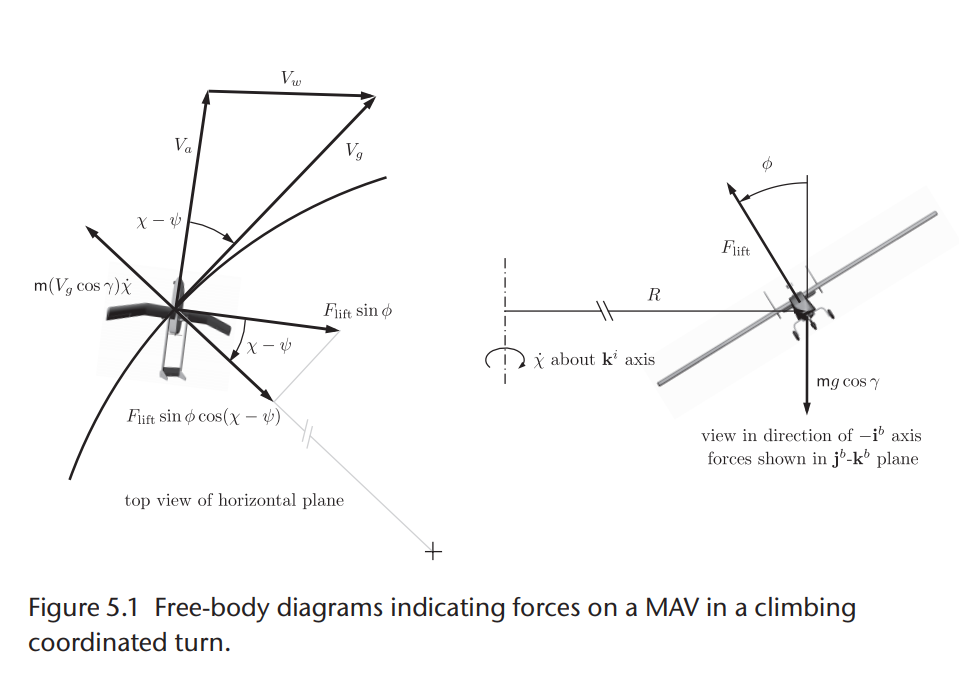
\includegraphics[width=0.8\textwidth]{pictures/5_1.png}
        \caption{爬升协调转弯MAV上的力}
        \label{fig:1}
    \end{figure}
    \par 作用在水平方向上的合力表示如下: 
    \begin{align}
        F_{lift} sin \phi cos (\chi - \psi) &= m \frac{v^{2}}{R} \nonumber \\
        &= m v \omega \nonumber \\
        &= m (V_{g} cos \gamma) \dot{\chi} 
        \label{equ:1}
    \end{align}
    其中, $F_{lift}$代表的是升力, $\gamma$ 代表的是飞行轨迹的角度, $V_{g}, \chi$ 分别表示的是地速度以及方向角. \textcolor{red}{向心加速度的表达式: $a_{n} = \frac{v^{2}}{R} = v \omega$}
    \par 离心力(The centrifugal force)计算的时候, 用到了在惯性坐标系$k^{i}$上的方向角变化率$\dot{\chi}$ 和 速度的水平分量 $V_{a}cos \gamma$
    \par 同样, 升力的垂直分量与重力在 $j^{b} - k^{b}$平面上的投影是等大反向的. 
    垂直方向上的合力为:
    \begin{equation}
        F_{lift} cos \phi = mg cos\gamma
        \label{equ:2}
    \end{equation}
    将等式\ref{equ:1}除以\ref{equ:2}得的 $\dot{\chi}$
    \begin{equation}
        \dot{\chi} = \frac{g}{V_{g}} tan \phi cos(\chi - \psi)
        \label{equ:3}
    \end{equation}
    等式\ref{equ:3}就是协调转弯的表达式. 
    \par 考虑到转弯半径等于 \textcolor{blue}{ $R = V_{g} \frac{cos \gamma}{\dot{\chi}}$}, 将上式代入半径中, 得到式子\ref{equ:4}. 在没有风或侧滑的情况下, 有\textcolor{red}{$V_{a} = V_{g}$和$\psi = \chi$}, 从而得到了式子\ref{equ:5}. 
    \begin{equation}
        R = \frac{V_{g}^{2} cos \gamma}{g tan \phi cos(\chi - \psi)} 
        \label{equ:4}
    \end{equation}
    \begin{equation}
        \dot{\chi} = \frac{g}{V_{g}} tan \phi = \dot{\psi} = \frac{g}{V_{a}} tan \phi
        \label{equ:5}
    \end{equation}
    \par 在 9.2 节中, 我们将要介绍 在有风的情况下 \textcolor{blue}{$ \dot{\psi} = \frac{g}{V_{a}} tan \phi$} 该式子也成立
    
    \section{Trim Conditions}
\end{document}